\newpage
\hypertarget{M2TSettingUp tex}{}
\subsection{Initializing the project}
\texHeader

{\bf update download so it includes a constraint file for \texttt{Dictionary}}

\begin{enumerate}

\item[$\blacktriangleright$] Your expanded \texttt{Dictionary} metamodel MOSL structure should resemble that found in Fig.~\ref{eclipse:startDictionary}. You'll
notice that it is accessing the \emph{Moca} framework by importing the \texttt{MocaTree} in \texttt{\_imports.mconf}.

\begin{figure}[htpb]
\begin{center}
  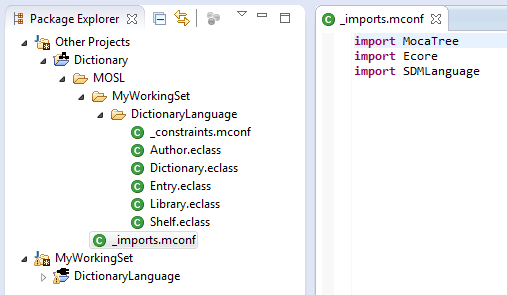
\includegraphics[width=0.8\textwidth]{eclipse_startingDictionary}
  \caption{figureCaption}
  \label{eclipse:startDictionary}
\end{center}
\end{figure}

\item[$\blacktriangleright$] Create a new \texttt{EPackage} named \texttt{DictionaryCodeAdpater}. It should include a \texttt{\_patterns} folder and
\texttt{\_constraints} file.

\item[$\blacktriangleright$] We'll need to create a metamodel to base our parser on, so create a new empty \texttt{EClass} in the new directory called
\texttt{Transformer}. Confirm your workspace resembles Fig.~\ref{eclipse:updatedDictionary}, then build your project to finish initilization.

\newpage

\begin{figure}[htpb]
\begin{center}
  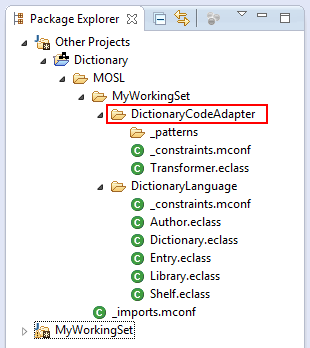
\includegraphics[width=0.5\textwidth]{eclipse_updatedDictionary}
  \caption{figureCaption}
  \label{eclipse:updatedDictionary}
\end{center}
\end{figure}

\end{enumerate}
